% =============================================================================
% MST (MCP-Skill-Tool) Architecture — Clean Rebuild
% Design language: classic academic block diagram, generous whitespace,
% clear visual hierarchy, no decorative shadows
% =============================================================================
\documentclass[tikz, border=10pt]{standalone}
\usepackage{tikz}
\usepackage{helvet}
\renewcommand{\familydefault}{\sfdefault}
\usetikzlibrary{arrows.meta, calc, fit, backgrounds}

% Okabe-Ito colorblind-safe palette
\definecolor{mcpblue}{HTML}{0072B2}
\definecolor{skillorange}{HTML}{E69F00}
\definecolor{toolgreen}{HTML}{009E73}
\definecolor{ink}{HTML}{1A1A1A}
\definecolor{subink}{HTML}{555555}

\begin{document}
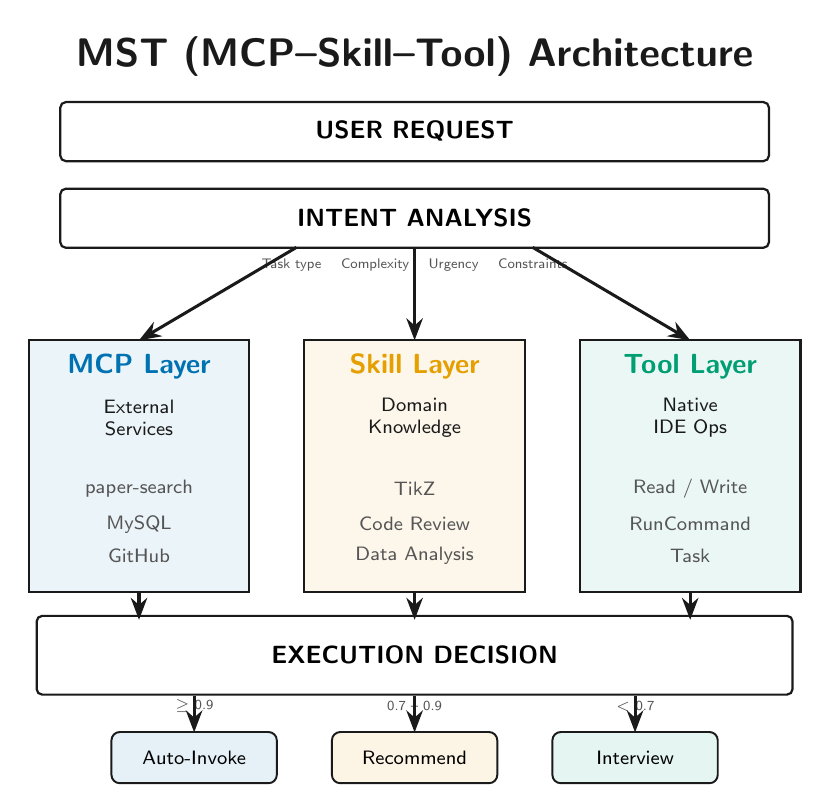
\begin{tikzpicture}[
    >=Stealth,
    arr/.style={->, line width=1.1pt, ink},
    every node/.style={font=\sffamily},
    % Pipeline header box
    header/.style={rectangle, rounded corners=2pt, draw=ink, line width=0.8pt, fill=white,
                   minimum width=9cm, minimum height=0.75cm, align=center, font=\small\bfseries},
    % Layer column box
    col/.style={rectangle, draw=ink, line width=0.8pt, fill=white,
                minimum width=2.8cm, minimum height=3.2cm, align=center,
                inner sep=8pt},
    % Small decision box
    decbox/.style={rectangle, rounded corners=3pt, draw=ink, line width=0.7pt,
                   minimum width=2.1cm, minimum height=0.65cm,
                   align=center, font=\scriptsize, fill=white},
    % Tiny confidence label
    cnf/.style={font=\tiny, text=subink}
]

% ---------- Title ----------
\node[font=\Large\bfseries, text=ink] at (0, 5.6) {MST (MCP--Skill--Tool) Architecture};

% ---------- Top pipeline ----------
\node[header] at (0, 4.65) (user) {USER REQUEST};
\node[header] at (0, 3.55) (intent) {INTENT ANALYSIS};
\node[cnf] at (0, 2.95) {Task type \quad Complexity \quad Urgency \quad Constraints};

% ---------- Three layer columns ----------
% MCP
\node[col, fill=mcpblue!8] at (-3.5, 0.4) (mcp) {};
\node[font=\bfseries, text=mcpblue] at (mcp.north) [yshift=-0.35cm] {MCP Layer};
\node[font=\scriptsize, text=ink, align=center] at ([yshift=-1.0cm]mcp.north) {External\\Services};
\node[font=\scriptsize, text=subink, align=center] at ([yshift=-1.9cm]mcp.north) {paper-search};
\node[font=\scriptsize, text=subink, align=center] at ([yshift=-2.35cm]mcp.north) {MySQL};
\node[font=\scriptsize, text=subink, align=center] at ([yshift=-2.75cm]mcp.north) {GitHub};

% Skill
\node[col, fill=skillorange!8] at (0, 0.4) (skill) {};
\node[font=\bfseries, text=skillorange] at (skill.north) [yshift=-0.35cm] {Skill Layer};
\node[font=\scriptsize, text=ink, align=center] at ([yshift=-1.0cm]skill.north) {Domain\\Knowledge};
\node[font=\scriptsize, text=subink, align=center] at ([yshift=-1.9cm]skill.north) {TikZ};
\node[font=\scriptsize, text=subink, align=center] at ([yshift=-2.35cm]skill.north) {Code Review};
\node[font=\scriptsize, text=subink, align=center] at ([yshift=-2.75cm]skill.north) {Data Analysis};

% Tool
\node[col, fill=toolgreen!8] at (3.5, 0.4) (tool) {};
\node[font=\bfseries, text=toolgreen] at (tool.north) [yshift=-0.35cm] {Tool Layer};
\node[font=\scriptsize, text=ink, align=center] at ([yshift=-1.0cm]tool.north) {Native\\IDE Ops};
\node[font=\scriptsize, text=subink, align=center] at ([yshift=-1.9cm]tool.north) {Read / Write};
\node[font=\scriptsize, text=subink, align=center] at ([yshift=-2.35cm]tool.north) {RunCommand};
\node[font=\scriptsize, text=subink, align=center] at ([yshift=-2.75cm]tool.north) {Task};

% ---------- Intent -> Layers (fan out) ----------
\draw[arr] (-1.5, 3.18) -- (-3.5, 2.0);
\draw[arr] (0, 3.18) -- (0, 2.0);
\draw[arr] (1.5, 3.18) -- (3.5, 2.0);

% ---------- Execution Decision ----------
\node[header, minimum width=9.6cm, minimum height=1.0cm] at (0, -2.0) (exec) {EXECUTION DECISION};

% Layers -> Exec (converge into top of exec box)
\draw[arr] (-3.5, -1.2) -- (-3.5, -1.55);
\draw[arr] (0, -1.2) -- (0, -1.55);
\draw[arr] (3.5, -1.2) -- (3.5, -1.55);

% ---------- Branches ----------
\node[decbox, fill=mcpblue!10] at (-2.8, -3.3) (auto) {Auto-Invoke};
\node[decbox, fill=skillorange!10] at (0, -3.3) (rec) {Recommend};
\node[decbox, fill=toolgreen!10] at (2.8, -3.3) (inter) {Interview};

% Confidence labels (between exec and branches)
\node[cnf] at (-2.8, -2.65) {$\geq$ 0.9};
\node[cnf] at (0, -2.65) {0.7 -- 0.9};
\node[cnf] at (2.8, -2.65) {$<$ 0.7};

% Exec -> Branches (fan out from bottom of exec)
\draw[arr] ($(exec.south) + (-2.8, 0)$) -- (-2.8, -2.98);
\draw[arr] (exec.south) -- (0, -2.98);
\draw[arr] ($(exec.south) + (2.8, 0)$) -- (2.8, -2.98);

\end{tikzpicture}
\end{document}
